\chapter{Locomotion in VR}
\label{sec:locomotion}




Curiosity and the thirst for exploration are an important part of human nature. It is not surprising how easy we tend to lose ourselves in large, open game worlds, spending countless hours on roaming around unknown terrain. Hence, locomotion  ever since had an important role in game design. And while this challenge is solved to a large extent in common digital games, locomotion techniques in virtual reality (VR) remain a large obstacle to this day.

This chapter discusses the challenges of VR locomotion and outlines a number of available solutions that allow the exploration of fictional worlds. We begin by looking at two important components of VR that one might also call the curse and blessing of such immersive setups: cybersickness and presence. In particular, we explain why common locomotion approaches, such as mouse and keyboard, are not viable in VR, and how the high degree of immersion allows the players to experience a feeling of being in the virtual world.

The main part of the chapter focuses on classifying the past and ongoing research on VR locomotion. We discuss a broad spectrum of possibilities to move in VR, ranging from stationary approaches relying on gamepads to advanced redirected walking techniques that trick our perception to enable unrestricted natural walking in a limited space. Finally, we propose a set of design guidelines to simplify the implementation of player locomotion in future VR games.




% ``parentheses''

\section{Presence and Cybersickness}

At present, VR technology is considered mainstream, and more and more manufacturers are putting effort into creating head-mounted displays (HMDs) at affordable prices. Such HMDs are capable of rendering stereoscopic images at HD resolutions for each eye while maintaining a high refresh rate (90 Hz or above). The hardware also tracks 
%at least 
the head orientation, which allows players to look around in VR like in real world and gather 
close-up experiences during gaming.

Players usually describe such impressions as a feeling of ``being there''~\cite{heeter1992being,lombard1997heart}. Other popular wordings often include the two terms \textit{presence} and \textit{immersion} --- sometimes in an interchangeable manner. Throughout the chapter, we utilize immersion~\cite{cairns2014immersion} when focusing on the technical quality of VR hardware ~\cite{Biocca:1995:IVR:207922.207926, sherman2002understanding}. In contrast, we use presence to describe how immersive setups affect our perception to make us believe that we are indeed in the virtual environment~\cite{slater2003note}. Hence, (game) researchers and developers often target the increase of presence when coming up with novel VR approaches, and VR locomotion is a prominent advocate for such presence-enhancing research~\cite{slater1995taking}. To measure presence, the most common methods include the Presence Questionnaire (PQ)~\cite{Witmer.2005} and the Igroup Presence Questionnaire (IPQ)~\cite{Schubert.2003, Schubert.2018}. In addition, the Immersive Tendencies Questionnaire (ITQ)~\cite{witmer1998measuring} can be administered before the actual survey to check participants' individual tendencies to get immersed in an activity or fiction. 


Unfortunately, the increase in players' perceived presence is not the only thing that an immersive setup entail. The produced realism imposes high demands on VR software and hardware regarding the human perception. Minor faults or technical issues, such as slightly offset locomotion or a sudden frame rate drop, can have severe consequences regarding the players' well-being and result in \textit{cybersickness}~\cite{stanney1997cybersickness,laviola2000discussion}. Other prominent terms often used in this context are \textit{simulator sickness}~\cite{kolasinski1995simulator} and \textit{motion sickness}~\cite{money1970motion,hettinger1992visually,ohyama2007autonomic}. In contrast to the manifold reasons of cybersickness, the main cause of simulator sickness is an incorrectly adjusted simulator~\cite{kennedy1989simulator} and can be regarded as a rather technical problem.




Cybersickness involves symptoms such as nausea, eye strain, and headaches. Roughly spoken, the main reason behind that negative phenomenon is a mismatch in our vestibulo-ocular system. Our vestibular system senses acceleration that ideally matches the visual input. When these signals do not match, the aforementioned symptoms are likely to occur~\cite{reason1975motion}. There exist three popular explanations~\cite{laviola2000discussion} for such an unwanted body reaction: poison theory, postural instability theory, and---the most prominent---conflict theory.  


Hettinger et al.~\cite{hettingerVection} also mentioned vection as a possible reason behind cybersickness. Vection describes the feeling of movement that relies only on our visual system and can be experienced when, e.g., we sit in a standing train and observe another train that is currently accelerating. Vection is influenced by several factors, including the field of view (FOV), the alignment and proximity of moving objects, and the optical flow rate. For instance, the combination of a large FOV and fast objects that account for a large proportion of players' view amplify the perceived vection and smooth the way to cybersickness. Hence, limiting the FOV is one of the possible approaches to reduce cybersickness~\cite{fernandes2016combating,lin2002effects}.


To conclude, we suggest keeping cybersickness in mind and to avoid cognitive mismatches where possible --- however, not at all costs, as ``sickness-save'', stationary scenes without any locomotion would potentially miss out on a wide range of benefits that VR has to offer. And sometimes, as shown by von Mammen et al.~\cite{von2016cyber}, games might even benefit from an artificially induced cybersickness. 


% von Mammen et al.~\cite{von2016cyber}



% ``parentheses''


\section{VR Locomotion Landscape}


We have seen that locomotion in VR is not just a way of transporting the player from A to B. Rather, locomotion strives to provide realistic, immersive experiences that increase the player's presence while working around cybersickness. In recent years, research~\cite{boletsis2017new} and the game industry~\cite{Habgood:2017:HLP:3130859.3131437} created a plethora of varying locomotion approaches. As often the case, there is no ``right'' answer which one to pick for your upcoming VR game. Hence, the main purpose of the following sections is to provide a rough overview and classification of available approaches and to serve as a starting ground for further research and development. In particular, we start by considering locomotion approaches that do not involve a physical movement of the player, before moving on to techniques that evolve around the idea of natural walking in VR. 




\subsection{Stationary Approaches}

Although HMDs can track head movements, only a subset of them is capable of tracking the global position of a player in the room. One also says that such setups support \textit{room-scale tracking}. One common approach is to utilize a set of base stations that emit infrared pulses, which are captured by the HMD to estimate the global position. Conversely, there is a considerable amount of HMDs that comes without room-scale support. Main reasons to omit such tracking are the lower costs and the increased portability. As such devices do not support the physical movement of the player, stationary locomotion techniques are required to allow the exploration of game worlds. Another reason for stationary approaches is the reduced fatigue, as players might even remain seated during a gaming session.





\subsubsection{Traditional I/O Approaches}

Existing games are sometimes ported to VR, be it to promote the title or to build on the success of the original game. In such cases, developers tend to take over the controls including locomotion to reduce the turnaround time and keep the familiar game UI. Hence, VR players are pushed towards desktop I/O, be it a keyboard~\cite{argelaguet2016giant}, a joystick~\cite{bozgeyikli2016locomotion}, or a gamepad~\cite{fernandes2016combating}. The advantage of the method is, without doubt, its simplicity regarding implementation and the familiarity to experienced players.

However, as we pointed out before, a cognitive mismatch between our vision system, i.e., seeing the motion via the HMD, and our vestibular system, i.e., remain stationary or even seated, can easily lead to cybersickness when using such approaches. Hence, we recommend to pay close attention to this issue when relying on traditional methods. As a partial remedy, developers might want to reduce the FOV, as, e.g., was done in Skyrim VR~\cite{SkyrimVR}. Another way would be to limit or disable continuous in-game player motion in favor of quick or discrete player movements~\cite{Habgood:2017:HLP:3130859.3131437} to reduce vection. The work of Medeiros et al.~\cite{medeiros2016effects} and Yao et al.~\cite{yao2014oculus} also confirmed the benefits of short, fast movements with no acceleration as one measure to combat cybersickness in such cases.

%Medeiros et al.~\cite{medeiros2016effects}
%Yao et al.~\cite{yao2014oculus}



\subsubsection{Teleportation}

If we take the idea of fast and short movements to the extreme, we will end up with a technique called the point and teleport locomotion approach~\cite{bozgeyikli2016point}. Players select a destination using a pointing device, e.g., a controller~\cite{7892303}, and are instantly teleported to that place, thus entirely removing the vection issues. Regarding cybersickness, this technique is more robust than traditional gamepad locomotion~\cite{frommel2017effects} and is being strongly encouraged by the majority of established VR systems such as the HTC Vive.





The targeting is often visualized by an arc that starts at the controller or the virtual hand representation and ends at the planned destination. On the one hand, the targeting is considered intuitive and robust. On the other hand, however, such implementation limits the travel distance to visible places that are not far away, and certain virtual environments might further limit the travel distance by exposing obstacles, such as trees or walls, that prevent players from targeting more distant locations. 
In addition, the displayed teleportation arc itself is a rather obstructive interface element that covers parts of the game world and might decrease players' perceived presence, if it does not blend in well with the setting. 
Another issue to be considered is the limited precision when teleporting to very close areas, as the displayed arc gets too compressed and is not very helpful for predicting the outcome. This uncertainty often results in numerous relocation attempts until the desired position is finally achieved.

The last drawback of teleportation is the reduced spatial orientation of players, which might also impact their experienced presence. Players need to reorient themselves after a relocation, which imposes an additional cognitive load. To overcome this obstactle, researchers propose to render previews of the destination area, or, as proposed by Bruder et al.~\cite{bruder2009arch}, utilize such previews as virtual portals where players have to pass through to reach their target. 

%Bruder et al.~\cite{bruder2009arch}


The described arc-based teleportation, although being recommended by hardware manufacturers, is still relatively uncommon in VR games. A more widespread variation of the technique is known as node-based teleportation~\cite{Habgood:2017:HLP:3130859.3131437}. This technique is based on predefined points of interest that could be represented by, e.g., an icon. In contrast to the arc-based method, players cannot pick their destination freely and can only travel between such nodes. The node selection is usually implemented by looking at a node and pressing a button. The subsequent teleportation process is often accompanied by a fading animation. This feature, in combination with a clever choice of node locations, allows to reduce player disorientation, but obviously limits the perceived freedom of exploration. 



% \subsubsection{Gestures}

% Ever since the introduction of the Microsoft Kinect, gesture-based interaction finally became mainstream and also entered the gaming area. In general, gestures are often considered natural and intuitive, which is likely to have a positive influence on the player experience and the perceived presence in VR. Accordingly, we can rely on gestures to perform locomotion---still not as intuitive as physical walking, but often more natural than steering ones avatar via a gamepad while remaining seated.

% For mainstream VR setups, i.e., HMDs including tracked controllers, the amount of supported gestures is usually limited to head and arm/hand movements. When we talk about head gestures, we refer, of course, primarily to gaze-based locomotion: players rotate their heads in the direction they want to walk~\cite{kitson2017comparing,cardoso2016comparison}. The actual walking speed can be either predefined or controlled by leaning the head forward or backward. This kind of locomotion has the crucial advantage of not requiring any additional interaction devices. Hence, this approach is often utilized in VR setups based on low-cost smartphone head mounts, such as the Google Cardboard, that have no alternative ways of gathering user input rather than tracking the head orientation. On the downside, the gaze-based locomotion is less suited for  games that require simultaneous interactions, e.g., aiming and shooting while moving. Accordingly, we often find this approach in exploration-only scenarios like virtual tours through exhibitions. Instead of moving the head only, one could also use the whole body as a kind of human joystick~\cite{harris2014human} and lean into the desired direction. However, such approaches require additional sensing hardware, e.g., a Wii balance board.

% One straightforward way to support player multitasking is to control the locomotion by arm or hand gestures. Two prominent examples for such gestures include tap and push as proposed by Ferracani et al.~\cite{ferracani2016locomotion}. Tapping~\cite{piumsomboon2013user} is performed by pointing with the index finger, i.e.,  players show in the direction they would like to walk. Pushing resembles more the control of a machine, i.e., one grabs a virtual lever by closing the hand and triggers the locomotion by translating the hand forward. In terms of performance, tapping turned out to be more efficient regarding collision avoidance. A physically more expressive way to control locomotion is to swing our arms~\cite{wilson2016vr,mccullough2015myo} to initiate translations in VR. In contrast to delicate finger recognition required for the aforementioned tapping gesture, such arm swings can be easily tracked via mainstream VR controllers.



% % ``parentheses''
% \subsection{Walking-Inspired Techniques}

% We started our exploration of the locomotion landscape by looking at traditional I/O approaches and transitioned to more natural user interaction in the form of gestures. However, the most natural way for us, humans, to explore our environment is to \textit{walk}. If you have ever witnessed a kid putting on a VR HMD for the first time, you have noticed that this kid will start moving right away, because that is our ``out of the box'' locomotion technique. Hence, we dedicate the second part of our overview to approaches that are based on natural walking---be it physical treadmills, redirected walking, or just walking in place.



% \subsubsection{Natural Walking}

% Without doubt, the most realistic movement in VR is based on physical walking, as this approach copies our real-world locomotion one to one. A significant amount of research has confirmed the resulting superior realism and the positive effect on the perceived presence~\cite{slater1995taking,usoh1999walking,ruddle2009benefits,waller2013sensory,ruddle2006efficient}. Furthermore, natural walking positively influences the cognitive map in large environments, as shown by Ruddle et al.~\cite{ruddle2011walking}. As our real and virtual movements can be perfectly matched using natural walking, the risk of cybersickness is also minimized.

% %Ruddle et al.~\cite{ruddle2011walking}

% Unfortunately, unrestricted natural walking is hardly achievable due to various reasons. First, the physical location of the player has to be estimated, i.e., additional tracking is necessary. Second, even if we can track the player, the physical room size imposes an insuperable obstacle: sooner or later, you will end up against a wall. And while the tracking issue is solved to a large extend in modern VR setups, the room limitation still persists. Later in the text, we will see diverse solutions to that problem that rely on tricking our perception or modifying and rescaling the virtual environment to ``fit'' the game world into our living room.

% In its pure form, natural walking is mainly used in combination with teleportation or other stationary locomotion. Players perform large transitions via teleport and then walk a small distance, e.g., one or two steps, to their precise destination. On paper, this combination removes the excessive number of relocations that happen in pure teleportation approaches. However, researchers and developers also noticed that teleportation plays the dominant role and players often tend to forego the option of doing some real steps, as switching and combining multiple locomotion approaches produces an increased cognitive load. Another possibility to apply natural walking without further modifications is to design game worlds that are smaller than our living rooms. It sounds too restrictive, but certain games work surprisingly well under such conditions---above all, we point readers to the popular genre of escape room games.


% \subsubsection{Walking in Place}

% % Usoh et al.~\cite{usoh1999walking}
% One possible way to bypass the room-scale limitation is to walk in place. Being based on natural, walking-like motions, this approach also enhances presence~\cite{slater1995taking, tregillus2016vr} and is easy to learn~\cite{usoh1999walking}. According to Usoh et al.~\cite{usoh1999walking}, walking in place is less immersive than natural walking, but both solutions outperform virtual locomotion approaches such as teleportation regarding the achieved feeling of presence.

% Walking in place is usually implemented by tracking the leg movements of the player, either with built-in tracking or via additional sensors~\cite{templeman1999virtual}. More sophisticated approaches are capable of deriving the correct walking speed by utilizing gait principles~\cite{wendt2010gud} to respond to variations in step frequency.



% \subsubsection{Physical Treadmills}

% One variation of in-place walking are treadmills that allow the players to move in a physical way. Combined with a HMD, players usually cannot distinguish such installations from real walking experiences. However, in contrast to a fitness studio, virtual worlds are hardly ever built in a linear way and players need the ability to change the walking direction.

% Hence, VR games require omni-directional treadmills~\cite{Darken:1997:OTL:263407.263550} or variations such as the omni-directional ball-bearing disc platform~\cite{huang2003omnidirectional}. Due to their spatial requirements and high costs, commercial omni-directional solutions such as the VirtuSphere~\cite{skopp2014pilot} did not find their way into our living rooms. A viable alternative is a stepper machine~\cite{bozgeyikli2016locomotion}, which is cheap, small, and easy to use. However, the walking direction has to be extracted from additional input, such as head orientation, potentially increasing the cognitive load.


\subsubsection{Redirected Walking}
In contrast to walking in place techniques, which address the room-scale limitation by completely avoiding that the player moves through the real room, other approaches enable natural walking by applying redirection or reorientation. 
The idea of redirected walking is to manipulate the player's movement in the virtual world by creating a mismatch between the real world locomotion and the translation in the game world. As a result, the perceived movement in the virtual world is more extensive than the player actually moves in the real world space \cite{razzaque2001redirected, razzaque2005redirected,steinicke2010}. % https://www.uni-muenster.de/imperia/md/content/psyifp/ae_lappe/freie_dokumente/tvcg09_mr.pdf 
While players do not notice the manipulation, they unconsciously compensate the offset by slightly repositioning and reorienting themselves. Hence, by manipulating translation, path curvature, and rotation, reorientation techniques can be used to keep players inside the boundaries of the tracked space without making them aware of the fact that they are actually walking in circles. 
Nescher et al.~\cite{nescher2014} and Paris et al.~\cite{paris2017} discuss different redirection methods and algorithms, providing further information how such techniques can be applied to VR games.

Redirection and reorientation techniques maintain the advantages of natural walking regarding high perceived presence, intuitiveness, and a low risk of cybersickness. However, though current approaches tackle the issue of space limitation to some extent, they still require a much larger space than is given in common living rooms and, thus, require further adaptations in that regard~\cite{Grechkin:2016:RDT:2931002.2931018, engel2008psychophysically, langbehn2016subliminal,bruder2009arch}. 
The demands of such techniques in terms of the VR setup and the implementation are considerably high.


%Aus GulliVR: Due to the required space, redirected walking is rarely used for living room sized VR setups, and requires further adaptations~\cite{Grechkin:2016:RDT:2931002.2931018, engel2008psychophysically, langbehn2016subliminal,bruder2009arch} to overcome that limitation. 



% können das auch vor multiscale nav schieben

%Redirected walking: The user walks freely inside a limited physical space, while being able to explore unlimited virtual environments by employing so-called redirection techniques. These techniques try to introduce an unnoticeable mismatch between the user’s real and virtual movements to compress the larger virtual environment into a limited tracking space [40,47].

%Reorientation: The user walks freely inside a limited physical space, while being able to explore unlimited virtual environments by employing so-called reorientation. The reorientation is achieved by modifying the rotational gain of the users, so they physically turn around when they meet the boundaries of the physical space, thus allowing for continued travel in both worlds [59].


\subsubsection{Multiscale Navigation}

Until now, the approaches we considered usually perform on a 1:1 ratio between the physical and the real world. In other words, the travelled distance in the physical room roughly corresponds our virtual footprint. An alternative way to deal with the room-scale limitation is rescaling of players and/or their motion~\cite{Bhandari:2017:LSW:3139131.3139133}. Note that world rescaling is equivalent to player rescaling. However, we strongly discourage altering the world size, i.e., the size of all objects, due to obvious performance reasons and, in worst case, floating point precision issues.

In research, the dynamic scaling of virtual environments is mostly used within multiscale virtual environments (MSVEs)~\cite{Zhang:2002:SIM:571878.571884}. For instance, such approaches can be utilized to explore the inner organs of virtual human representations~\cite{kopper2006design}. Hereby, the current scale can be set either manually by the player or computed automatically based on current task or location. As shown by Argelaguet et al.~\cite{argelaguet2016giant}, automatic scaling is often more predictable for developers and allows to optimize rendering parameters to reduce diplopia or cybersickness.

In games research, a recent example of player rescaling is a locomotion technique called \textit{GulliVR}~\cite{Krekhov:2018:GVRA}. The approach allows players to turn into giants on demand and cover large distances in just a few steps. At first glance, the idea is similar to a common flying approach, as both variants share the same camera position and velocity. However, flying is known for its severe cybersickness due to the cognitive mismatch of physical and virtual movement speeds. In contrast, GulliVR increases the interpupillary distance as part of the whole-body rescaling process, which has two effects. First and foremost, the cybersickness is removed as players feel like they are walking as giants (no mismatch) and not like they are artificially floating or flying. Second, players perceive the environment from above as a miniature world, which opens up novel design possibilities~\cite{cmentowski2019outstanding}.


\section{Design Implications}




Locomotion in VR has a huge impact on the failure or success of a game. A well-chosen technique is able to enhance the player experience and help players to immerse even more in the fictional worlds. On the downside, technical issues or cognitive mismatches can easily render a game unplayable due to a significant amount of introduced cybersickness. Not surprisingly, our high-level recommendation is to design locomotion in a way that minimizes the risks of cybersickness and maximizes the perceived presence. Ideally, we would choose natural walking for most cases, but, unfortunately, the room-scale limitation forces us to consider alternatives and handle respective trade-offs.

For that reason, we recommend enforcing a decision regarding locomotion quite early in the development process, as certain approaches have a considerable interplay with other game mechanics, such as object interaction, quest locations, world size, etc. As a starting point for such decision making, we summarized the mentioned locomotion methods in Figure~\ref{fig:overview}. Please note that such overviews rely on certain over-generalizations, e.g., not all gamepad-based techniques are causing cybersickness. However, we feel that a condensed summary might be helpful, especially when designing a VR game for the first time. Furthermore, we propose the following questions to be asked during the VR game design process with respect to locomotion:

\textbf{\textit{What is my target audience?}} The canonical question for almost any kind of decision making. We emphasize three aspects of this question. First, how exhausting is the locomotion allowed to be? This depends on age and the overall target group, as well as the type of the game, i.e., it might be an exergame or something meant for relaxation/recovery. Second, how long are the players meant to play the game at a time? This aspect also determines how physically straining the locomotion is allowed to be. Third, what hardware setups do our players have? In other words, are we designing for Google Cardboard that only tracks head orientation or can we assume room-scale tracking? In particular, we are limited to stationary approaches if we do not have access to the player position.


\begin{figure}[t]
\centering
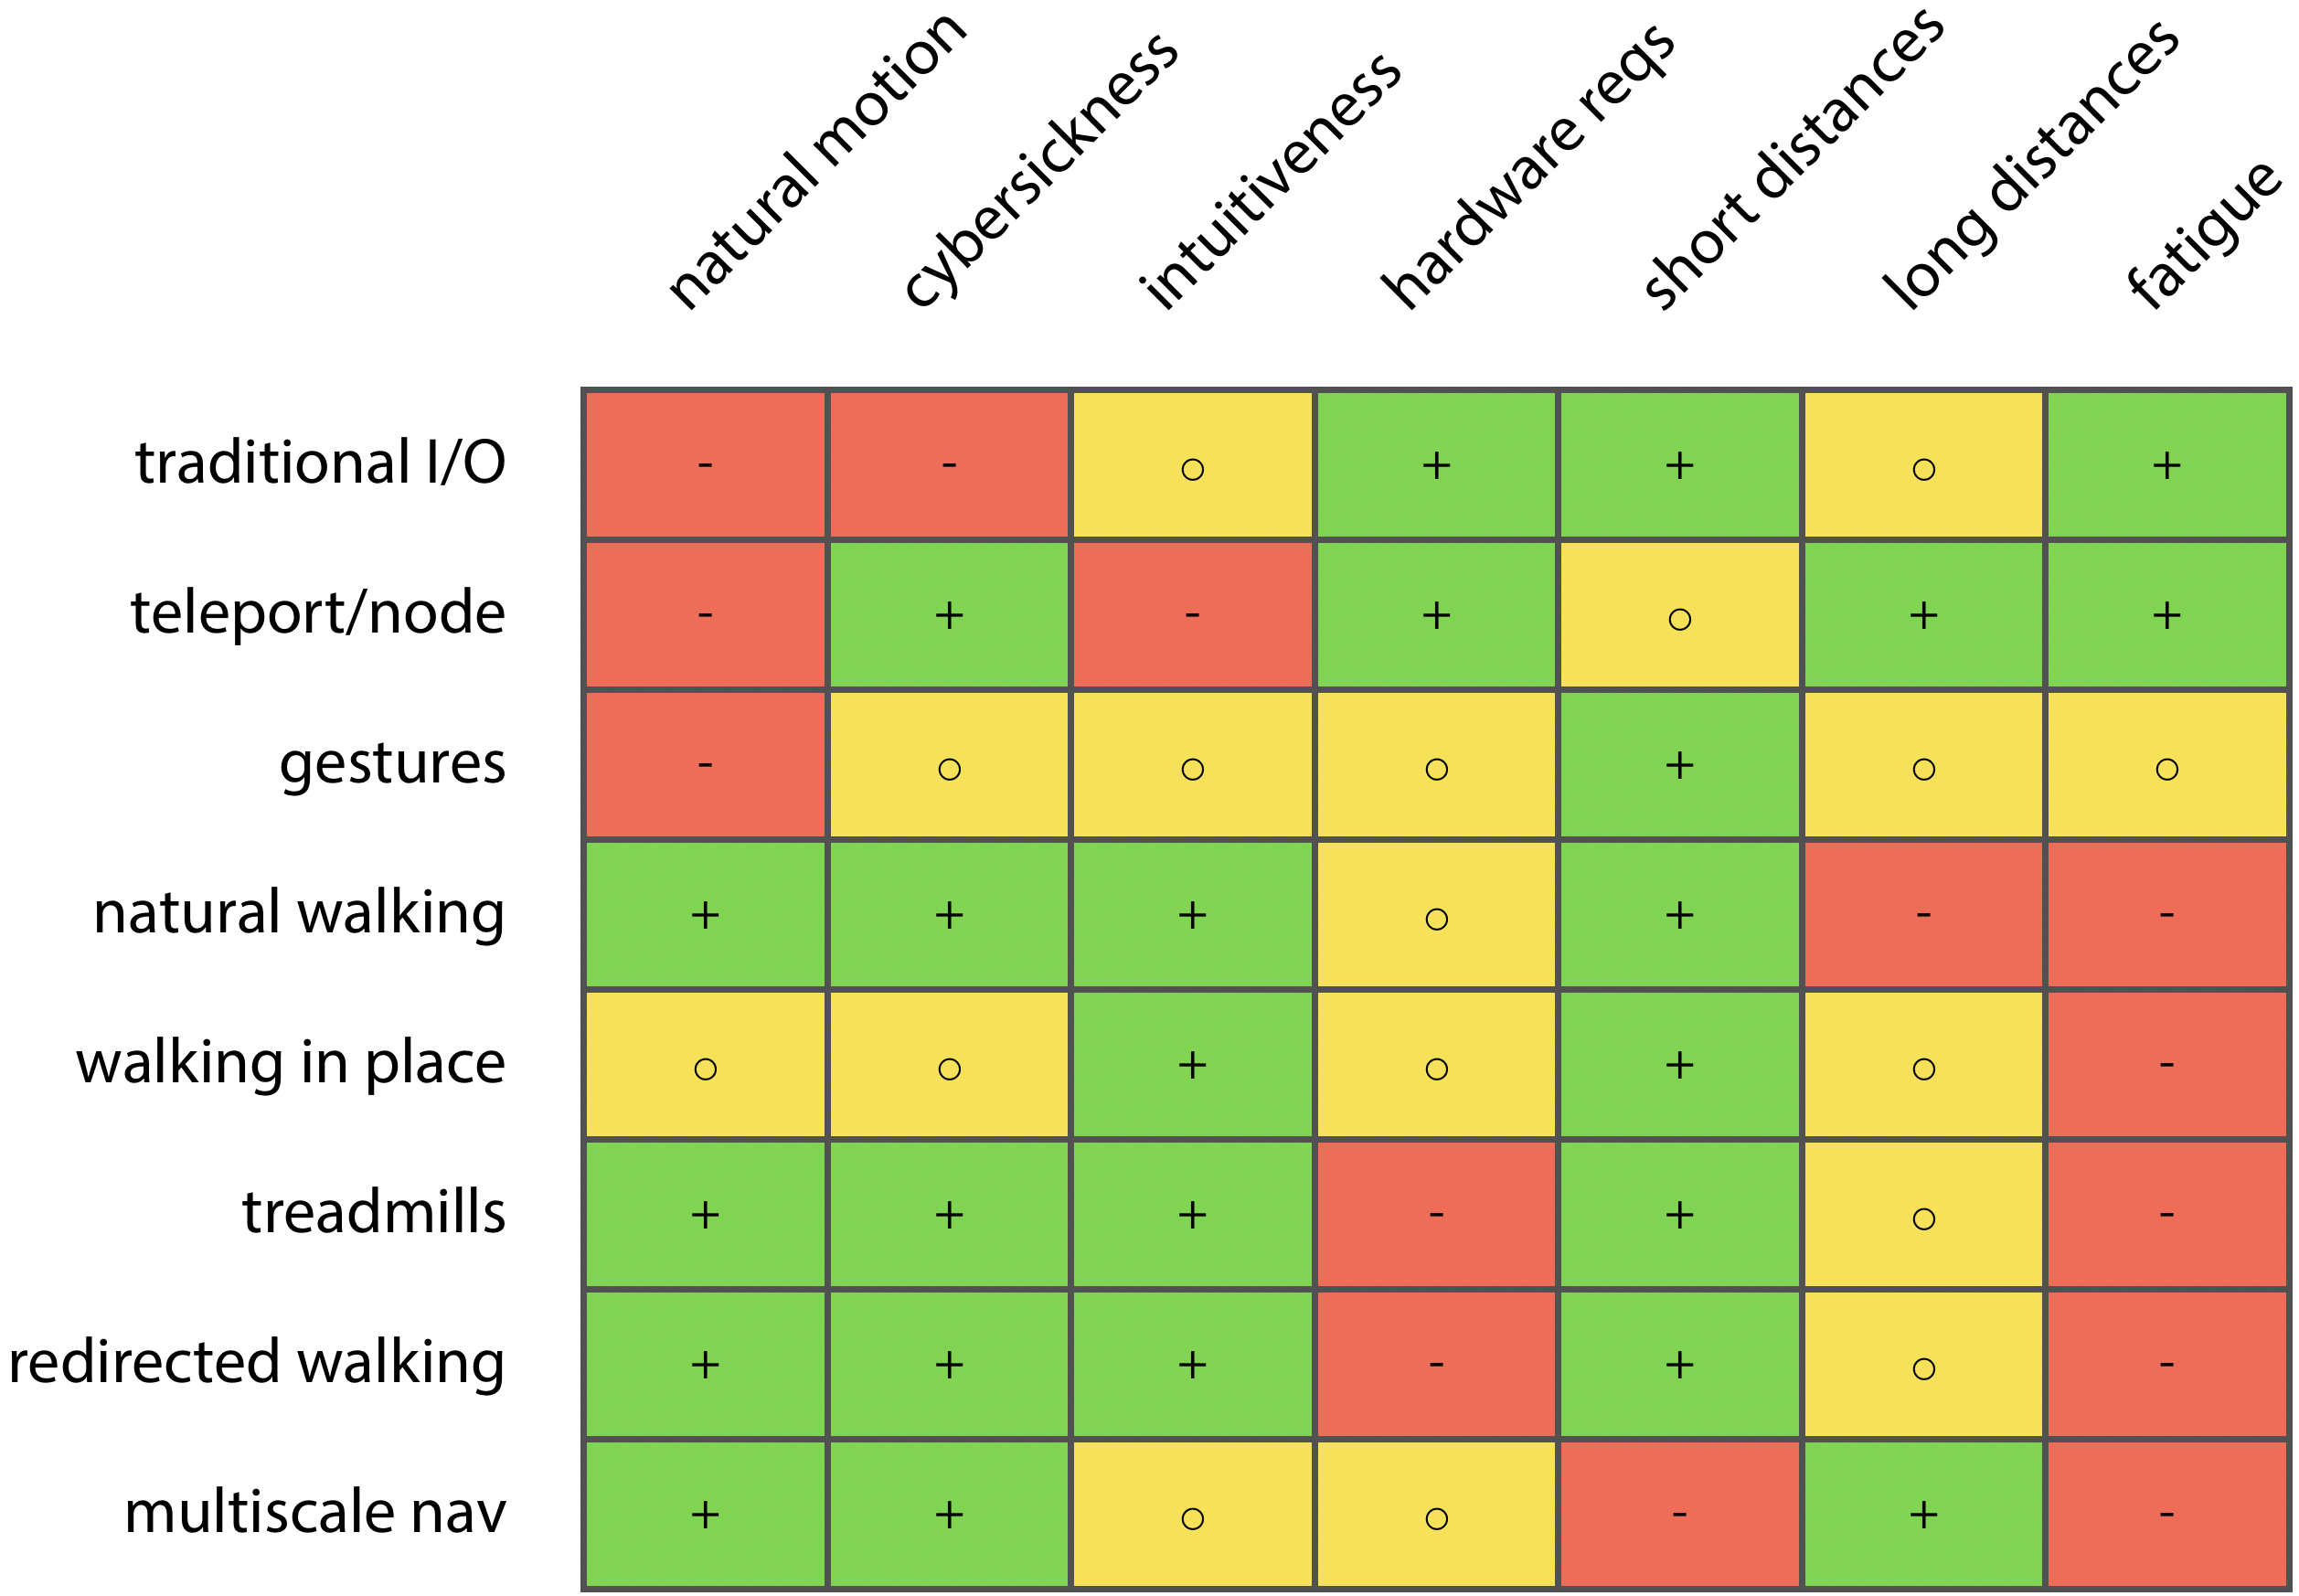
\includegraphics[width=1.0\columnwidth]{content/images/chapter14_figure1.jpg}
\caption{An overview of VR locomotion techniques including their benefits and drawbacks. Green color (+) means that this attribute is a known advantage of the technique, yellow ($\circ$) stands for limited value, and red (-) is rather a disadvantage.}
\label{fig:overview}
\end{figure}


\textbf{\textit{How important is exploration?}} In general, games with a heavy focus on exploration and player movement benefit a lot from realistic, well-constructed locomotion approaches that allow a free and natural journey through the virtual world. Conversely, if the main emphasis of the game is on aiming and shooting, a node-based teleportation technique with carefully predefined locations might be more efficient. Furthermore, the overall size of the virtual world should be considered, as some of the techniques excel at short distances, whereas other approaches are designed to cover large distances in a short amount of time. Taken to the extreme, certain game genres, such as escape rooms, might even consider to rely only on natural walking by fitting the virtual environment completely into the living room.


\textbf{\textit{What else happens during locomotion?}} This question is also related to the main focus of the game. Certain techniques, such as gaze-based locomotion, limit the amount of concurrent activities and are less suited for games in which players need to perform additional interactions while walking. The overall effort required for locomotion---be it mental or physical---also impacts the general pace of the game. In other words, fast-paced games might rather benefit from an instant, node-based teleportation rather than forcing players to physically run through their living rooms or spending precious seconds while aiming with the arc-based teleportation approach.


Again, these questions are meant as a starting point. In combination with the overview in Figure~\ref{fig:overview}, this kind of reasoning might be helpful to establish a well-suited locomotion technique early on and to take full advantage of virtual reality gaming.


